\documentclass[11pt,a4paper]{article}
\usepackage{lmodern}

\usepackage{amssymb,amsmath}
\usepackage{ifxetex,ifluatex}
\usepackage{fixltx2e} % provides \textsubscript
\ifnum 0\ifxetex 1\fi\ifluatex 1\fi=0 % if pdftex
  \usepackage[T1]{fontenc}
  \usepackage[utf8]{inputenc}
\else % if luatex or xelatex
  \ifxetex
    \usepackage{mathspec}
    \usepackage{xltxtra,xunicode}
  \else
    \usepackage{fontspec}
  \fi
  \defaultfontfeatures{Mapping=tex-text,Scale=MatchLowercase}
  \newcommand{\euro}{???}
\fi
% use upquote if available, for straight quotes in verbatim environments
\IfFileExists{upquote.sty}{\usepackage{upquote}}{}
% use microtype if available
\IfFileExists{microtype.sty}{%
\usepackage{microtype}
\UseMicrotypeSet[protrusion]{basicmath} % disable protrusion for tt fonts
}{}
\usepackage[lmargin=2.5cm,rmargin=2.5cm,tmargin=2.5cm,bmargin=2.5cm]{geometry}

% Figure Placement:
\usepackage{float}
\let\origfigure\figure
\let\endorigfigure\endfigure
\renewenvironment{figure}[1][2] {
    \expandafter\origfigure\expandafter[H]
} {
    \endorigfigure
}

%% citation setup
\usepackage{csquotes}

\usepackage[backend=biber, maxbibnames = 99, style = apa]{biblatex}
\setlength\bibitemsep{1.5\itemsep}
\addbibresource{R_packages.bib}
\bibliography{references.bib}
\usepackage{color}
\usepackage{fancyvrb}
\newcommand{\VerbBar}{|}
\newcommand{\VERB}{\Verb[commandchars=\\\{\}]}
\DefineVerbatimEnvironment{Highlighting}{Verbatim}{commandchars=\\\{\}}
% Add ',fontsize=\small' for more characters per line
\usepackage{framed}
\definecolor{shadecolor}{RGB}{248,248,248}
\newenvironment{Shaded}{\begin{snugshade}}{\end{snugshade}}
\newcommand{\AlertTok}[1]{\textcolor[rgb]{0.94,0.16,0.16}{#1}}
\newcommand{\AnnotationTok}[1]{\textcolor[rgb]{0.56,0.35,0.01}{\textbf{\textit{#1}}}}
\newcommand{\AttributeTok}[1]{\textcolor[rgb]{0.77,0.63,0.00}{#1}}
\newcommand{\BaseNTok}[1]{\textcolor[rgb]{0.00,0.00,0.81}{#1}}
\newcommand{\BuiltInTok}[1]{#1}
\newcommand{\CharTok}[1]{\textcolor[rgb]{0.31,0.60,0.02}{#1}}
\newcommand{\CommentTok}[1]{\textcolor[rgb]{0.56,0.35,0.01}{\textit{#1}}}
\newcommand{\CommentVarTok}[1]{\textcolor[rgb]{0.56,0.35,0.01}{\textbf{\textit{#1}}}}
\newcommand{\ConstantTok}[1]{\textcolor[rgb]{0.00,0.00,0.00}{#1}}
\newcommand{\ControlFlowTok}[1]{\textcolor[rgb]{0.13,0.29,0.53}{\textbf{#1}}}
\newcommand{\DataTypeTok}[1]{\textcolor[rgb]{0.13,0.29,0.53}{#1}}
\newcommand{\DecValTok}[1]{\textcolor[rgb]{0.00,0.00,0.81}{#1}}
\newcommand{\DocumentationTok}[1]{\textcolor[rgb]{0.56,0.35,0.01}{\textbf{\textit{#1}}}}
\newcommand{\ErrorTok}[1]{\textcolor[rgb]{0.64,0.00,0.00}{\textbf{#1}}}
\newcommand{\ExtensionTok}[1]{#1}
\newcommand{\FloatTok}[1]{\textcolor[rgb]{0.00,0.00,0.81}{#1}}
\newcommand{\FunctionTok}[1]{\textcolor[rgb]{0.00,0.00,0.00}{#1}}
\newcommand{\ImportTok}[1]{#1}
\newcommand{\InformationTok}[1]{\textcolor[rgb]{0.56,0.35,0.01}{\textbf{\textit{#1}}}}
\newcommand{\KeywordTok}[1]{\textcolor[rgb]{0.13,0.29,0.53}{\textbf{#1}}}
\newcommand{\NormalTok}[1]{#1}
\newcommand{\OperatorTok}[1]{\textcolor[rgb]{0.81,0.36,0.00}{\textbf{#1}}}
\newcommand{\OtherTok}[1]{\textcolor[rgb]{0.56,0.35,0.01}{#1}}
\newcommand{\PreprocessorTok}[1]{\textcolor[rgb]{0.56,0.35,0.01}{\textit{#1}}}
\newcommand{\RegionMarkerTok}[1]{#1}
\newcommand{\SpecialCharTok}[1]{\textcolor[rgb]{0.00,0.00,0.00}{#1}}
\newcommand{\SpecialStringTok}[1]{\textcolor[rgb]{0.31,0.60,0.02}{#1}}
\newcommand{\StringTok}[1]{\textcolor[rgb]{0.31,0.60,0.02}{#1}}
\newcommand{\VariableTok}[1]{\textcolor[rgb]{0.00,0.00,0.00}{#1}}
\newcommand{\VerbatimStringTok}[1]{\textcolor[rgb]{0.31,0.60,0.02}{#1}}
\newcommand{\WarningTok}[1]{\textcolor[rgb]{0.56,0.35,0.01}{\textbf{\textit{#1}}}}
\usepackage{longtable,booktabs}
\usepackage{graphicx}
\makeatletter
\def\maxwidth{\ifdim\Gin@nat@width>\linewidth\linewidth\else\Gin@nat@width\fi}
\def\maxheight{\ifdim\Gin@nat@height>\textheight\textheight\else\Gin@nat@height\fi}
\makeatother
% Scale images if necessary, so that they will not overflow the page
% margins by default, and it is still possible to overwrite the defaults
% using explicit options in \includegraphics[width, height, ...]{}
\setkeys{Gin}{width=\maxwidth,height=\maxheight,keepaspectratio}
\ifxetex
  \usepackage[setpagesize=false, % page size defined by xetex
              unicode=false, % unicode breaks when used with xetex
              xetex]{hyperref}
\else
  \usepackage[unicode=true, linktocpage = TRUE]{hyperref}
\fi
\hypersetup{breaklinks=true,
            bookmarks=true,
            pdfauthor={Sunyoung Ji},
            pdftitle={Signing Up New Fathers: Do paternity Establishment Initiatives Increase Marriage, Patental Investment, and Child Well-Being?},
            colorlinks=true,
            citecolor=blue,
            urlcolor=blue,
            linkcolor=magenta,
            pdfborder={0 0 0}}
\urlstyle{same}  % don't use monospace font for urls
\setlength{\parindent}{0pt}
\setlength{\parskip}{6pt plus 2pt minus 1pt}
\setlength{\emergencystretch}{3em}  % prevent overfull lines
\setcounter{secnumdepth}{5}

%%% Use protect on footnotes to avoid problems with footnotes in titles
\let\rmarkdownfootnote\footnote%
\def\footnote{\protect\rmarkdownfootnote}

%%% Change title format to be more compact
\usepackage{titling}

% Create subtitle command for use in maketitle
\newcommand{\subtitle}[1]{
  \posttitle{
    \begin{center}\large#1\end{center}
    }
}

\setlength{\droptitle}{-2em}
  \title{Signing Up New Fathers: Do paternity Establishment Initiatives
Increase Marriage, Patental Investment, and Child Well-Being?}
  \pretitle{\vspace{\droptitle}\centering\huge}
  \posttitle{\par}
\subtitle{Causality and Programme Evaluation}
  \author{Sunyoung Ji}
  \preauthor{\centering\large\emph}
  \postauthor{\par}
  \predate{\centering\large\emph}
  \postdate{\par}
  \date{today}


%% linespread settings

\usepackage{setspace}

\onehalfspacing

% Language Setup

\usepackage{ifthen}
\usepackage{iflang}
\usepackage[super]{nth}
\usepackage[ngerman, english]{babel}

%Acronyms
\usepackage[printonlyused, withpage, nohyperlinks]{acronym}
\usepackage{changepage}

% Multicols for the Title page
\usepackage{multicol}


\usepackage{longtable}

\begin{document}

\selectlanguage{english}


%\maketitle

\begin{titlepage}
  \noindent\begin{minipage}{0.6\textwidth}
	  \IfLanguageName{english}{University of Duisburg-Essen}{Universit\"at Duisburg-Essen}\\
	  \IfLanguageName{english}{Faculty of Business Administration and Economics}{Fakult\"at f\"ur Wirtschaftswissensschaften}\\
	  \IfLanguageName{english}{Chair of Econometrics}{Lehrstuhl f\"ur \"Okonometrie}\\
  \end{minipage}
	\begin{minipage}{0.4\textwidth}
	  \begin{flushright}
  	  \vspace{-0.5cm}
      \IfLanguageName{english}{\includegraphics*[width=5cm]{Includes/duelogo_en.png}}{\includegraphics*[width=5cm]{Includes/duelogo_de.png}}
	  \end{flushright}
	\end{minipage}
  \\
  \vspace{1.5cm}
  \begin{center}
  \huge{Signing Up New Fathers: Do paternity Establishment Initiatives
Increase Marriage, Patental Investment, and Child Well-Being?}\\
  \vspace{.25cm}
  \Large{Causality and Programme Evaluation}\\
  \vspace{0.5cm}
  \large{Term Paper}\\
  \vspace{1cm}
  \large{
  \IfLanguageName{english}{Submitted to the Faculty of \\ Business Administration and Economics \\at the \\University of Duisburg-Essen}{Vorgelegt der \\Fakult\"at f\"ur Wirtschaftswissenschaften der \\ Universit\"at Duisburg-Essen}\\}
  \vspace{0.75cm}
  \large{\IfLanguageName{english}{from:}{von:}}\\
  \vspace{0.5cm}
  Sunyoung Ji\\
  \end{center}
  %\vspace{2cm}
  \vfill
  \hrulefill

  \noindent\begin{minipage}[t]{0.3\textwidth}
  \IfLanguageName{english}{Reviewer:}{Erstgutachter:}
  \end{minipage}\\
  \begin{minipage}[t]{0.7\textwidth}
  \hspace{1cm}Prof.~Martin Karlsson, Ph.D, Chair of Health Economics 
  \end{minipage} \\
    \begin{minipage}[t]{0.7\textwidth}
  \hspace{1cm}TA Nikolaos Prodromidis. M.Sc., Chair of Health Economics
  \end{minipage}

  \noindent\begin{minipage}[t]{0.3\textwidth}
  \IfLanguageName{english}{Deadline:}{Abgabefrist:}
  \end{minipage}\\
  \begin{minipage}[t]{0.7\textwidth}
  \hspace{1cm}01. 10. 2022
  \end{minipage}

  \hrulefill

  \begin{multicols}{1}

  Name:

  Matriculation No.:

  E-Mail:

  Study Path:

  Semester:

  \columnbreak

  Sunyoung Ji

  229979

  sunyoung.ji@gmail.com

  M.Sc. Econometrics

  \nth{5}

 

  \end{multicols}

\end{titlepage}

\newgeometry{top=2cm, left = 5cm, right = 2.5cm, bottom = 2.5cm}


\pagenumbering{Roman}
{
\hypersetup{linkcolor=black}

\setcounter{tocdepth}{3}
\tableofcontents
}

\newpage
\listoffigures
\addcontentsline{toc}{section}{List of Figures}

%\newpage
\listoftables
\addcontentsline{toc}{section}{List of Tables}

\section*{List of Abbreviations}
\addcontentsline{toc}{section}{List of Abbreviations}

\begin{adjustwidth}{1.5em}{0pt}

\begin{acronym}[dummyyyy]
 \acro{ECTSCP}{European Credit Transfer System Credit Point}
 \acro{lasso}{Least Absolute Shrinkage and Selection Operator}
 \acro{pcr}{Principal Components Regression}
 \acro{pls}{Partial Least Squares}
 \acro{RMSE}{Root Mean Squared Error}
 \acroplural{LRG}[LRG]{laengefristige Refinanzierungsgeschaefte}

%Falls eine Abkuerzung in der Mehrzahl nicht einfach auf "s" endet muss das speziell eingestellt werden.
% \acro{slmtA}{super lange mega tolle Abkuerzung} %Einzahl
 %\acroplural{slmtA}[slmtAs]{super lange mega tolle Abkuerzungen} %Mehrzahl
 \acro{dummyyyy}{dummyyy}
\end{acronym}

\end{adjustwidth}

\restoregeometry

\newpage
\pagenumbering{arabic}
\hypertarget{introduction}{%
\section{Introduction}\label{introduction}}

In-hospital Voluntary Paternity Establishment (IHVPE) is implemented for
children in unmarried families. The expected main effects of IHVPE was
improving child well-being and parental investments by making easy
to establish paternity. It does require less costs and less time than
the legal paternity establishment that includes complicated process with
the court system and DNA testing. According to the author Maya
Rossin-Slater (2017), IHVPE increases paternity, but decreases
marriages. The effects on father involvements and child well-being is
seem to close to zero or even negative value, in other words, this
policy hardly achieves its purpose. The author mentions the reason is
the influence of IHVPE to parental marriages. Fathers who would get
married with child mother in the absence of IHVPE decide to be not
married. Thereby, children could not be provided with private health
insurance by their biological father's employees, and father would spend
less time with their children and provide less support as they live
separately from their children. To analyze these treatments effects of
IHVPE empirically, the author conduct the quasi-experimental variation
in the timing of IHVPE program initiation across stats and years. The
analyses of the CPS-CSS data are on the individual level with the
statistical model below:

\begin{equation}
Y_{isty} = \beta_{0} + \beta_{1}  IHVPE_{sy} +
\gamma'  X_{isty} + \phi'  C_{st} + \mu_{s} + \alpha_{y} + \delta_{s}
 y + \epsilon_{isty}
\end{equation}

for each mother i, in state s,
in survey year t, with a youngest child born in year y. \(Y_{isty}\) is
an outcome of interest, \(X_{isty}\) individual maternal and chlid
characteristics, and coefficients \(\beta_1\)is a measure the effect of
the existence of IHVPE in the child's state and year of birth on the
\(Y_{isty}\). The details of variables are in Appendix A.1. The
identifying assumptions for (1) are uncorrelation between the state-year
variation in the timing of IHVPE implementation and other unobserved
time-varying determinants of the outcomes of interest, and common trend
assumption that the treatment and comparison states would have had
similar trends in outcomes of interest in the absence of IHVPE
introduction. The result that can be derived from this author's study is
very interesting. I wanted to recheck that IHVPE is not successful
policy by applying a new method to the existed dataset. To replicate
Rossin-Slater's study, the causal forests is desirable, first, it allows
to deal with high dimensional data. CPS-CSS dataset contains total
67-dimensional space, and in each replication, the number of variables
is from 28 to 29 including covariate, outcomes, cluster and treatment
variables. Moreover, the causal forests provide heterogeneous treatment
effects: which/How much subgroups vary treatments effects. Lastly, under
some assumptions, causal forests offer a pointwise consistent estimate
and accurate asymptotic variance and have asymptotically Gaussian and
centered sampling distribution which is informative on the statistical
inference. The paper proceeds as follows. Chapter 2 introduces CPS-CSS
data and the use of causal forests as an empirical methods. Chapter 3
shows steps for building a replication model, main results and
evaluation of the model.

\hypertarget{data-current-population-survey-child-support-supplements-cps-css}{%
\section{Data: Current Population Survey Child Support Supplements
(CPS-CSS)}\label{data-current-population-survey-child-support-supplements-cps-css}}

Rossin-Slater use the biannual March/April matched CPS-CSS to analyze
the effects of IHVPE on parental marriage, birth father's involvements
and child well-being. The dataset consists of 48,119 moms that
were surveyed both in March annual demographic file and in the monthly
April CPS from 1994 to 2008. For the replication, I used the same
subsets with original paper. Variable details are given in Appendix 1.

\hypertarget{replication-with-causal-forests}{%
\section{Replication with Causal
Forests}\label{replication-with-causal-forests}}

\hypertarget{introduction-of-the-causal-forests}{%
\subsection{Introduction of the Causal
Forests}\label{introduction-of-the-causal-forests}}

To estimate causal effects of IHVPE, I apply the causal forests which
are the machine learning method that captures heterogeneous treatment
effects. In the causal forests, each regression tree is created by first
drawing a random subsample of the data. The individuals in the subsample
are then split into subgroups (``leaves'') based on covariate values,
where the splits are defined by minimizing some loss function such as
the root mean squared error. The process is then repeated and averaged
over B trees, resulting in random forest that can be used to predict
\(Y_i\) for a particular covariate combination \(X_i = x\). The
estimation with the causal forests proceeds with
\texttt{grf\ (generalized\ random\ forests)} package in R. \texttt{grf}
provides non-parametric methods for heterogeneous treatment effects
estimation for forest-based statistical estimation and inference
(Tibshirani, et al.).

\hypertarget{identification-assumptions}{%
\subsection{Identification Assumptions}\label{identification-assumptions}}

This replication with causal forests estimation assumes below:
\begin{itemize}
\item Conditional unconfoundedness: $(Y_i^1, Y_i^0) \perp D_i \mid X_i$ \\
\item Stable Unit Treatment Value Assumption (SUTVA): $Y_i=Y_i^0+D_i(Y_i^1-Y_i^0)$ \\
\item Overlap assumption: for all $x \in supp(X_i), 0<P(D_i=1 \mid X_i=x)<1$, $P(D_i = 1 \mid X_i = x) = e(x)$ \\
\item Exogeneity of covariates
\end{itemize}

To satisfy conditional unconfoundedness, I create selection index which sorts confounded variables by selecting variables with high importance. More detail is mentioned in Chapter 3.3.2. step4. Overlap assumption is satisfied by positive probability of treatment for each $X_i$. It can be conformed by the histogram of $e(x) = \(\mathbb{E}[W_i\mid X=x]\) which is provided in Chapter 3.5.2






\hypertarget{replication}{%
\subsection{Replication}\label{replication}}

\hypertarget{variables}{%
\subsubsection{Variables}\label{variables}}

The estimation of treatment effects of IHVPE in this paper consists of 4
replications. Each replication estimates treatment effects (\(W_i\)) on
parental marriages, child private health insurance in all parents
groups, child private health insurance in families that do not live
with child supports from biological fathers respectively.

\begin{longtable}{l|p{10cm}}
\caption{Treatments Variables in Each Replications} \\
\hline
\textbf{Replications} & \textbf{Treatment Variables($Y_i$)}    \\
\hline
\endfirsthead % Erster Kopf zu Ende
% Definition des Tabellenkopfes auf den folgenden Seiten
\caption{Treatments Variables in Each Replications (continued)}\\
\hline
\textbf{Replications} & \textbf{Treatment Variables($Y_i$)}  \\
\hline
\endhead % Zweiter Kopf ist zu Ende
\multicolumn{3}{r}{Continued on the next page.}\\
\endfoot
\hline
\multicolumn{3}{r}{End of table.} \\
\endlastfoot
Rep 1 & mother who is married to child's father \\
Rep 2 & child who has private health insurance coverage \\
Rep 3 & child who has private health insurance coverage \\
Rep 4 & father who covered any gifts, clothes, food, childcare, or
medical expenses \\
\bottomrule()
\end{longtable}

It is assumed that the moms in the same state
could arbitrary correlated within the a state, since the years of IHVPE
initiation are vary between different states. Thus, state FIPS is
assigned as a cluster in the replication. When it comes to the
covariates, it is devided into 4 groups:

\begin{longtable}{l|p{10cm}}
\caption{Treatments Variables in Each Replications} \\
\hline
\textbf{Covariates\(X_i\)} & \textbf{Variables}    \\
\hline
\endfirsthead % Erster Kopf zu Ende
% Definition des Tabellenkopfes auf den folgenden Seiten
\caption{Treatments Variables in Each Replications (continued)}\\
\hline
\caption{Treatments Variables in Each Replications} \\
\hline
\endhead % Zweiter Kopf ist zu Ende
\multicolumn{3}{r}{Continued on the next page.}\\
\endfoot
\hline
\multicolumn{3}{r}{End of table.} \\
\endlastfoot
Households controls & mother's age, education, race, total number of
children in a household, child's gender, age \\
States controls & unemployment rate, poverty rate, minimum wages,
percentage of population on medicaid \\
CS controls & universal wage withholding, license revocation for
non-payment, joint custody law, log total expenditures on child support
enforcement \\
welfare controls & AFDC waiver, TANF, EITC \\
\bottomrule()
\end{longtable}

The treatment variable indicating implication of IHVPE is a dummy
variable from 1 to 0.

\hypertarget{Replication-Steps}{%
\subsubsection{Replication Steps}\label{Replication-Steps}}
\begin{itemize}
\item \textbf{Step 1: Estimate $m(x) = \mathbb{E}[Y_i\mid X=x]$ and $e(x) = \mathbb{E}[W_i\mid X=x]$} \\
I train regression forests with outcome variables and the treatment in each replications to make out-of-bag estimates of $m(x)$ and $e(x)$ to grow the causal forests through \\
$$\hat{\tau} = \frac{\sum_{i=1}^N \alpha_{i}(x)(Y_{i} - \hat{e}^{(-i)}(X_{i}))}{\sum_{i=1}^N \alpha_{i}(x)(W_{i}- \hat{e}^{(-i)}(X_{i}))^2 }$$\\
, where $\alpha_{i}(x)$ is a data-adaptive kernel that measures how often individual training example falls in the same leaf as the the test points x (Athey and Wagger, 2019).
\\

\item \textbf{Step 2: Grow a causal forest with $m(x)$ and $e(x)$ with tuning parameters} \\
I tune all possible parameters by cross-validation with the tuning 
option \texttt{tune\_parameters} of \texttt{grf}. \\
\item \textbf{Step 3: Train the causal forests on all covariates} \\
\item \textbf{Step 4: Train the new causal forests with important covariate variables}  \\
Through the random forests, I check the importance of all variables, then make the selection index including only variables with bigger importance than the mean of overall importance. By training the causal forests with only important variables in low signal situations, I can eliminate features that may be confounded. \\
\item \textbf{Step 5: Estimate Average Treatment effects (ATE) of the causal forests}
\end{itemize}


\hypertarget{results}{%
\subsection{Results}\label{results}}


\begin{longtable}{l|l|l|l|l{6cm}}
\caption{Results of Replications} \\
\hline
\textbf{.} & \textbf{Rep 1}& \textbf{Rep 2} & \textbf{Rep 3}  & \textbf{Rep 4}   \\
\hline
\endfirsthead % Erster Kopf zu Ende
% Definition des Tabellenkopfes auf den folgenden Seiten
\caption{Results of Replications (continued)}\\
\hline
\caption{Results of Replications} \\
\hline
\endhead % Zweiter Kopf ist zu Ende
\multicolumn{3}{r}{Continued on the next page.}\\
\endfoot
\hline
\multicolumn{3}{r}{End of table.} \\
\endlastfoot
Rossin-Slater & -0.0281 (0.0088) & -0.0263 (0.0101) & . & 0.0161 (0.0290)\\
ATE & -0.0148 (0.0064) & -0.0151 (0.0040) & -0.0281 (0.0143) & 0.0389 (0.0196)\\
RATE & -0.0185 (0.0073) & 0.0077 (0.0044) & 0.0137 (0.0214) & 0.0418 (0.0127)\\
\bottomrule()
\end{longtable}

In table 3, Rep1, Rep2, Rep3 and Rep4 are replications to estimate treatment effects of IHVPE on marriage, private health insurance for children in all households, private health insurance for children who are not living with their biological father and child support from birth father to children who are not living with their birth father respectively. The first row shows coefficients of treatment effects of IHVPE on each outcome of interest which estimate by Rossin-Slater. The second and third rows illustrates average treatment effect and rank-weighted average treatment effects that offered by replication. The rank-weighted average treatment effect is a weighted sum of targeting operator characteristics. The Targeting Operating Characteristic (TOC) is a curve comparing the benefit of treating only a certain fraction (q) of units to the overall average treatment effect. A weighted sum of TOC identifies prioritization rules that effectively targets treatment (Tibshirani, et al.).
In summary, the results from replications reflects that the treatment effects of IHVPE on marriage and child private health insurance are less significant than the results from Rossin-Slater's paper. On the other hand, Replication 4 shows effect on any child support from birth dad increases after treatment(IHVPE).


\begin{itemize} 
\item Rank-Weighted Average Treatment Effects (RATE)
\begin{figure}
\centering
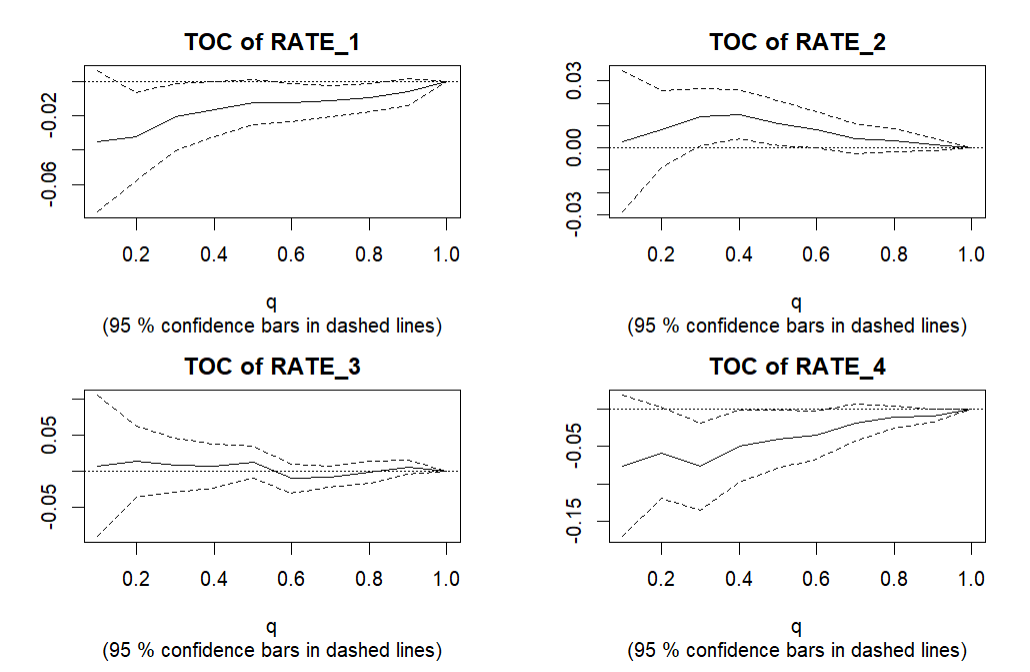
\includegraphics[width = 15cm] {rate_toc}
\hfill
\caption{Targeting Operator Characteristics}
\label{rate_toc}
\end{figure}
\end{itemize}

Table 4 introduces a measure of the quality of the estimates of treatment heterogeneity, $D_i = (\hat{\tau}^{(-i)}(X_i) - \bar{\tau})(W_i - \hat{e}^{(-i)}(X_i))$, where $\bar{\tau}$ is the average of the treatment effect estimates. If estimates equals to 1, the mean of forest prediction is accurate. In Table 5, the estimates are coefficients of the differential forest prediction. It implies that the heterogeneity estimates from the forests are well calibrated, if it is 1 as estimates in Table 4. The p-value of differential forest prediction in Table 5 acts as omnibus test for the existence of heterogeneity. The p-value which is greater than 0 means there is heterogeneity (Tibshirani, et al.).




\hypertarget{model-evaluation}{%
\subsection{Model Evaluation}\label{model-evaluation}}
\hypertarget{Evaluation-of-Treatment-Heterogeneity}{%
\subsubsection{Evaluation of Treatment Heterogeneity}\label{Evaluation-of-Treatment-Heterogeneity}}
The best linear predictor method(Chernozhukov, et al., 2018)fits CATE as a linear function of the out-of-bag causal forest estimates(Athey and Wager, 2019). \texttt{grf} provies \texttt{test\_calibration} function that computes the best linear fit of the target estimates using the forest prediction and the mean forest prediction(Tibshirani, et al.). \\




As Table 4 show, the estimates quite close to 1, especially Rep2 and Rep4. Thus, the causal forest models in the replications predict good the average of the treatment effect estimates. In Table 5, Though estimates are far from 1, except for Rep2, the p-values of Rep2, Rep3 and Rep4 are greater than 0, therefore, I can reject the null hypothesis, that is, there is heterogeneity.
\newpage
\begin{longtable}{l|l|l|l|p{2cm}}
\caption{Best Linear Predictor Method 1} \\
\hline
\textbf{Replications} & \textbf{estimate}& \textbf{std.err} & \textbf{t.value}  & \textbf{p.value}   \\
\hline
\endfirsthead % Erster Kopf zu Ende
% Definition des Tabellenkopfes auf den folgenden Seiten
\caption{Best Linear Predictor Method: mean.forest.prediction (continued)}\\
\hline
\textbf{Replications} & \textbf{estimate}& \textbf{std.err} & \textbf{t.value}  & \textbf{p.value}   \\
\hline
\endhead % Zweiter Kopf ist zu Ende
\endfoot
\hline
\multicolumn{3}{r}{End of table.} \\
\endlastfoot
Rep1 & 0.8255 & 0.5309 & 1.5548 & 0.0600\\
Rep2 & 1.0608 & 0.9583 & 1.1070 & 0.1342\\
Rep3 & 1.5048 & 0.4433 & 3.3944 & 0.0003\\
Rep4 & 1.0505 & 0.2989 & 3.5149 & 0.0002
\bottomrule()
\end{longtable}




\begin{longtable}{l|l|l|l|p{2cm}}
\caption{Best Linear Predictor Method 2} \\
\hline
\textbf{Replications} & \textbf{estimate}& \textbf{std.err} & \textbf{t.value}  & \textbf{p.value}   \\
\hline
\endfirsthead % Erster Kopf zu Ende
% Definition des Tabellenkopfes auf den folgenden Seiten
\caption{Best Linear Predictor Method: differential.forest.prediction (continued)}\\
\hline
\textbf{Replications} & \textbf{estimate}& \textbf{std.err} & \textbf{t.value}  & \textbf{p.value}   \\
\hline
\endhead % Zweiter Kopf ist zu Ende
\endfoot
\hline
\multicolumn{3}{r}{End of table.} \\
\endlastfoot
Rep1 & 1.1624 & 0.7811 & 1.4881 & 0.0684\\
Rep2 & -0.0424 & 0.4609 & -0.0919 & 0.5366\\
Rep3 & -10.7970 & 2.2546 & -4.7888 & 1.0000\\
Rep4 & -10.2456 & 1.9367 & -5.2903 & 1.0000
\bottomrule()
\end{longtable}

\hypertarget{Evaluation of Overlap}{%
\subsubsection{Evaluation of Overlap}\label{Evaluation of Overlap}}

The overlap assumption requires a positive probability of treatment for each $X_i$. None of the estimated propensity scores $e(x)$ should be one or zero. $e(x)$ in each replication has the positive range of values, however, Not a few values are shown to be close to 1. This part will need to be improved for a more robust model in the future.

\begin{figure}
\centering
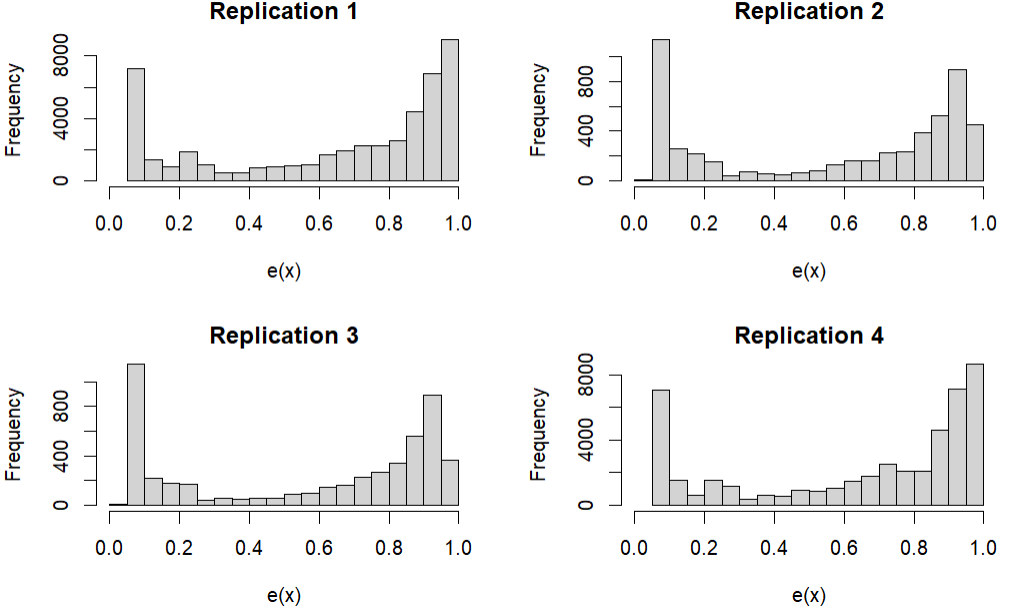
\includegraphics[width = 15cm] {overlap}
\hfill
\caption{Histogram of e(x)}
\label{overlap}
\end{figure}

\hypertarget{conclusion}{%
\section{\texorpdfstring{Conclusion
\label{chap:conc}}{Conclusion }}\label{conclusion}}
The results of Replications can be summarized as follows. 
1) The impact of IHVPE on marriage reduction and child private health insurance is less. 2) The impact of IHVPE on any child support provided by the birth father has increased significantly from 0.0161 in Rossin-Slater's paper to 0.0389. In other words, IHVEPE encourages birth fathers to invest more in their children by improving the relationship between fathers and children. In contrast, there is a limit to IHVPE's influence because most of the private health insurance is provided by employees to their legal families. Despite the imperfections of the current model, IHVPE is not large, but I think it works to some extent.


\pagebreak

\textbf{\textit{\HUGE{Refrences}}} \\

Athey, Susan & Wager, Stefan. (2019). Estimating Treatment Effects with Causal Forests: An Application. Observational Studies. 5. 37-51. 10.1353/obs.2019.0001. \\

Rossin-Slater, Maya. doi: 2017. "Signing Up New Fathers: Do Paternity Establishment Initiatives Increase Marriage, Maya Rossin-Slater, Parental Investment, and Child Well-Being?" American Economic Journal: Applied Economics, 9 (2): 93-130. doi:10.1257/app.20150314\\

Victor Chernozhukov & Vira Semenova, 2018. "Simultaneous inference for Best Linear Predictor of the Conditional Average Treatment Effect and other structural functions," CeMMAP working papers CWP40/18, Centre for Microdata Methods and Practice, Institute for Fiscal Studies. <https://ideas.repec.org/p/ifs/cemmap/40-18.html>

\newpage

\cleardoublepage
\appendix
\setcounter{table}{0}
\setcounter{figure}{0}
\renewcommand{\thetable}{A\arabic{table}}
\renewcommand{\thefigure}{A\arabic{figure}}

\newgeometry{top=2.5cm, left = 2cm, right = 2cm, bottom = 2.5cm}

\hypertarget{appendix}{%
\section{Appendix}\label{appendix}}

\hypertarget{description-of-relevant-variables}{%
\subsection{\texorpdfstring{Description of Relevant Variables
\label{app:A}}{Description of relevant Variables }}\label{description-of-relevant-variables}}

\begin{longtable}{l|l|p{6cm}}
\caption{Description of Relevant Variables} \\
\hline
\textbf{Variable} & \textbf{Controls} & \textbf{Description}    \\
\hline
\endfirsthead % Erster Kopf zu Ende
% Definition des Tabellenkopfes auf den folgenden Seiten
\caption{Description of Relevant Variables (continued)}\\
\hline
\textbf{Variable} & \textbf{Controls} & \textbf{Description}    \\
\hline
\endhead % Zweiter Kopf ist zu Ende
\multicolumn{3}{r}{Continued on the next page.}\\
\endfoot
\hline
\multicolumn{3}{r}{End of table.} \\
\endlastfoot
momage1 & household controls & mother aged \<20 at time of childbirth \\
momage2 & household controls & mother aged 20-24 at time of childbirth \\
momage3 & household controls & mother aged mother aged 25-34 at time of childbirth \\
momage4 & household controls & mother aged 35-44 at time of childbirth \\
momeduc1 & household controls & mother with \< high school education \\
momeduc2 & household controls & mother with high school degree \\
momeduc3 & household controls & mother with some college \\
momwhite & household controls & mother is non-Hispanic white \\
momblack & household controls & mother is non-Hispanic black \\
momhispanic & household controls & mother is Hispanic \\
ch\_male & household controls & child is male \\
child\_age & household controls & child's age in years \\
father\_outsidehh & household controls & child's age in years \\
totkids & household controls & total number of kids in the household \\
\hline 



unemp\_rate\_lag1 & state controls & last year's unemployment rate \\
pov\_rate\_lag1 & state controls & last year's poverty rate \\
state\_minwage\_lag1 & state controls & last year's state-level minimum wage \\
pct\_welf\_recp\_lag1 & state controls & last year's percentage of population receiving welfare \\
\hline




wage\_withold & cs controls & universal wage withholding implemented in state/year \\
new\_hires & cs controls & New Hires Directory implemented in state/year \\
license\_revoke & cs controls & License revocation for non-payment implemented in state/year \\
joint\_custody & cs controls & joint custody law implemented in state/year \\
log\_CS\_exp\_lag & cs controls & log total expenditures on child support enforcement last year \\
\hline



waiver & welfare controls & AFDC waiver implemented in state/year \\
tanf & welfare controls & TANF implemented in state/year \\
eitc & welfare controls & state EITC program implemented in state/year \\
\hline


state & cluster & state EITC  \\
\hline


child\_hcovpriv & potential outcomes & child has private health insurance coverage \\
married\_tobiodad & potential outcomes & mother is married to child's father \\
\hline




any\_hosp\_pat & treatment & IHVPE exists in state and year
\label{tab_var}
\end{longtable}


\end{document}
